\section{Equilibrium \& Comparative Statics}
\label{sec:section3} 
\subsection{Steady State Equilibrium and Approximation}\label{sec:section3.1} 
Following from the above, I now present a refined definition for the steady state equilibrium of the market: 
\begin{definition}
    A Steady State Equilibrium is defined by a triplet $(\mu^*, \omega^*, \Psi^*)$ such that:
    \begin{enumerate}
        \item $ \mu^*(\theta,b) \text{ attains } V_m(\theta,b), \; \forall\, \theta, b \in \Theta \times \mathcal{B}_m$, given $\omega^*,\Psi^*$
        \item $ \omega^*(\theta,b) \text{ attains } V_w(\theta,b), \; \forall\, \theta, b \in \Theta \times \mathcal{B}_w$, given $\mu^*,\Psi^*$
        \item $\Psi^*$ satisfies Equations \ref{eq:ss1}, \ref{eq:ss2}, and \ref{eq:ss3} given the strategy profile $(\mu^*, \omega^*)$
    \end{enumerate} 
\end{definition}

Intuitively, the above definition establishes two conditions that must be satisfied by an equilibrium market configuration. Firstly, it must be the case that $\mu^*$ and $\omega^*$ are mutual best responses given the platform state $\Psi^*$; however, as previously outlined, a necessary and sufficient condition for this would have them each solve the sex-specific MDP. This essentially rules out mixed-strategy equilibria which would never be optimal for either MDP. Furthermore, in line with mean-field game theory literature, a \textit{consistency check} is imposed by the third condition, which requires that the platform steady-state to which agents are best-responding with $(\mu^*,\omega^*)$ is sustained. Overall, the above equilibrium concept demands \textit{partially rational expectations} from agents, as ....

Although formal proofs of existence and uniqueness for steady-state equilibria are outside the scope of this paper, I instead rely on computational procedures\footnote{The code required to reproduce all analysis presented in this paper is fully accessible under the GitHub repository \texttt{patohdzs/project-tinder}} to approximate equilibria under various exogenous configurations to shed some light on the insights provided by the theoretical model and its ability to replicate and explain stylized empirical facts. I propose two computational procedures to solve for model equilibria, both of which involve framing the recurrence relation presented in Proposition 1, as well as Equations \ref{eq:ss1}, \ref{eq:ss2}, and \ref{eq:ss3}, as a system of $2(|\mathcal{B}_m|+|\mathcal{B}_w|+1)$ non-linear equations, denoted by $\mathbf{E}(\mu,\omega,\Psi)$. From here, the first procedure utilizes a modified version of Powell's method, as per the MINPACK 1 routine \citep{more1980user}, whilst the second one solves the following least squares problem:

\begin{equation*}
    \begin{split} 
        \mu^*, \omega^*, \Psi^* = \arg\min_{\mu,\omega,\Psi} \quad &  ||\mathbf{E}(\mu,\omega,\Psi)||^2 \quad \textrm{s.t.} \quad  \mu, \omega  \in [0,1] 
    \end{split}
\end{equation*}
 

\subsection{Best Response Analysis}\label{sec:section3.2} 
Using the computational procedures outlined above, a number of insights can be uncovered related to how exogenous parameters affect an agent's best-response swiping strategy. The first parameter I analyse is the discount factor, which represents the probability of remaining inside the platform for an additional time period, but is often interpreted as the representative agent's patience level. To determine the effects that changes in the discount factor have on the best-response policy, I computed the latter over a range of different values for $\delta$ (using an arbitrary set of exogenous parameters), with results shown in \autoref{fig:discount-cs}. Evidently, as the agent becomes less patient, they `lower their standards' for potential matches in the platform, shifting their swiping curve downwards. 

\begin{figure}[ht] 
    \centering
    \caption{Comparative Statics on the Discount Factor}
    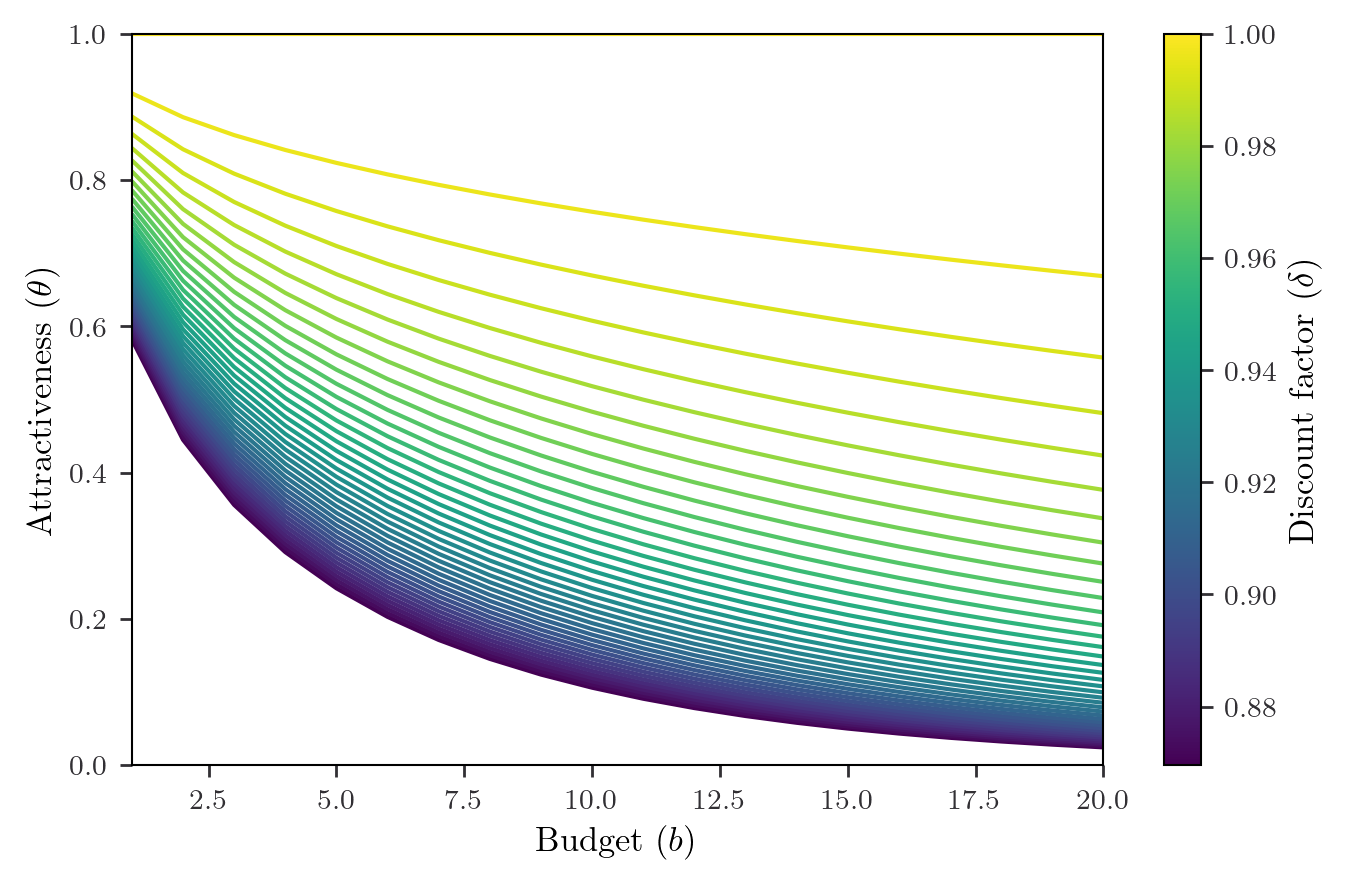
\includegraphics{discount-cs.png}
    \label{fig:discount-cs}
\end{figure}

%An alternative interpretation of this effect considers the view of a geometrically-distributed platform lifetime process (as explained in \autoref{sec:section2.1}). Under this interpretation, an agent's platform lifetime is of ${1}/{1-\delta}$ periods in expectation, meaning that swiping caps significantly higher than this number render the constraint non-binding, thus reverting the game to the trivial case where all agents swipe right in all periods.

Another interesting parameter to examine is the absolute risk aversion of agents, which I choose to interpret as their `desperateness' for matching in the platform. In the platform, risk-averse agents prefer a higher chance of matching (even if these matches yield relatively lower payoffs), whilst risk-loving agents prefer to wait around and save their swipes for high-yield candidates. To perform comparative statics on this parameter, I fix a CARA utility function for agents, with parameter $r$ denoting the Arrow-Pratt coefficient for absolute risk aversion. With these preferences, I then compute the optimal swiping rule for various different values of $r$ and an arbitrary set of exogenous parameters, with results for this shown on \autoref{fig:risk-cs}. From this, it is evident that as agents become `more desperate' for matches, implied by rising absolute risk aversion, they lower their standards for right-swiping on a candidate, thus shifting their swiping curve downwards (as one would intuitively expect).

\begin{figure}[ht]
    \centering
    \caption{Comparative Statics on Absolute Risk Aversion}
    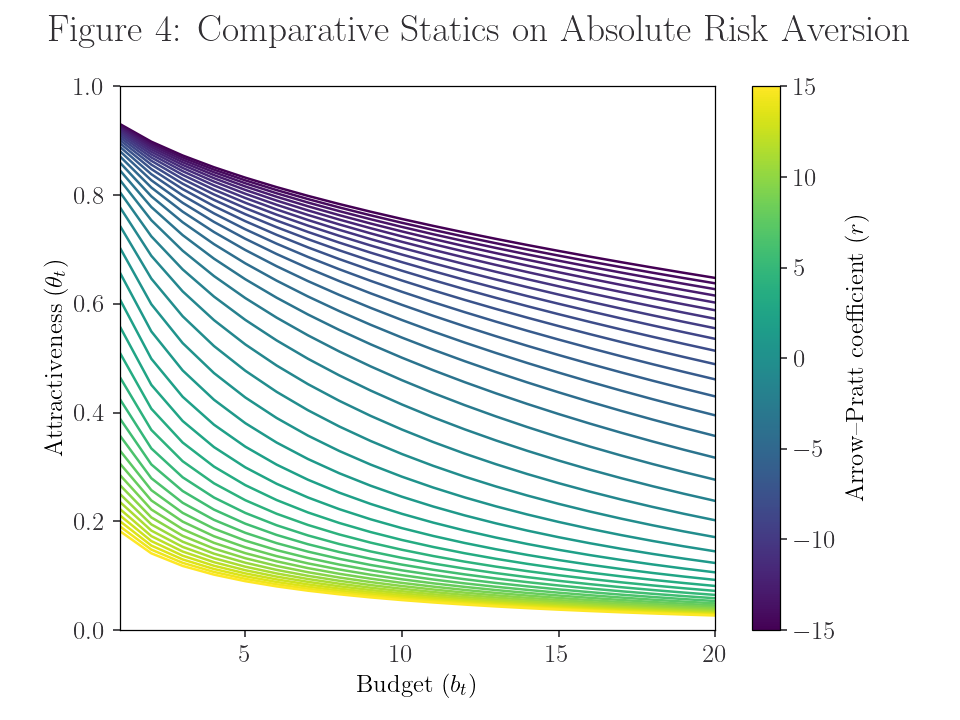
\includegraphics{risk-cs.png}
    \label{fig:risk-cs} 
\end{figure}

\subsection{Market Configuration Analysis}\label{sec:section3.3} 
Finally, I perform comparative statics at the platform level to determine how different factors affect market configurations. This is especially important as it considers not only the effects on best-responses for one sex, but also how these affect the market as a whole through the aggregate state. More specifically, I focus the aforementioned `Fast-Swiping Males' puzzle, which investigates the discrepancy in swiping and matching rates between men and women, and present three possible explanations for how the model developed in this paper can replicate and explain this outcome. The first explanation concerns differential inflows for both men and women, which occur exogenously within my model but are in line with empirical findings, which . To asses the market configurations arising from of this situation, I compute the model equilibria under a 6:1 ratio between arrival rates $\lambda_m$ and $\lambda_w$. The results for this are shown in \autoref{fig:mkt-cs}, highlighting three main insights for this scenario. 

\begin{figure}[ht]
    \centering
    \caption{Market Configuration Under Differential Agent Inflows}
    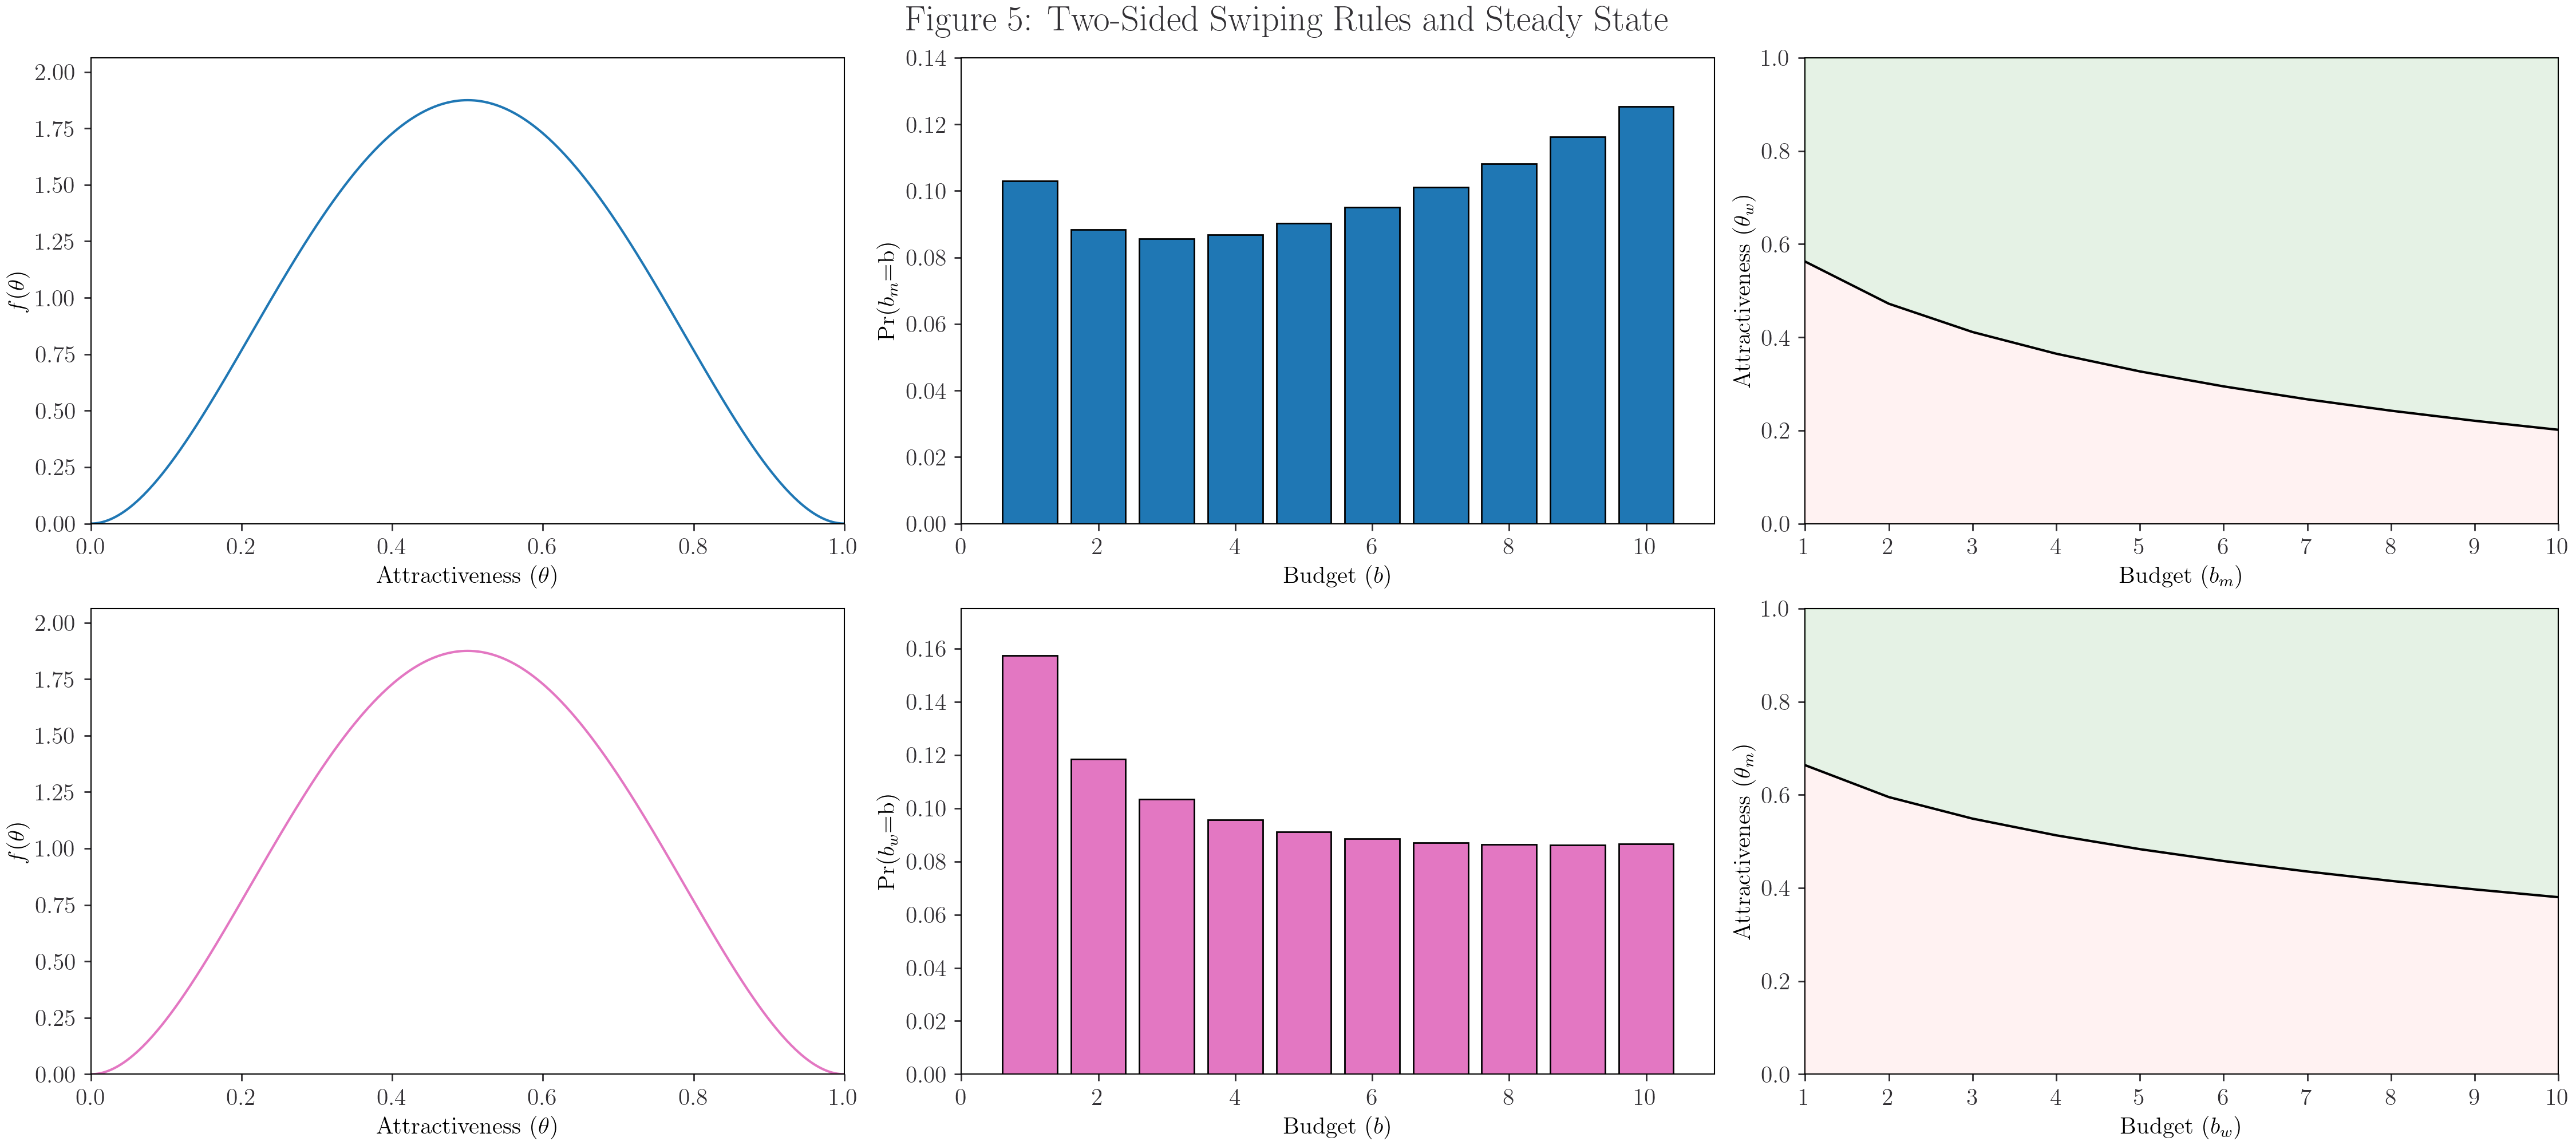
\includegraphics{mkt-cs.png}
    \label{fig:mkt-cs} 
\end{figure} 

Firstly, under differential agent inflows, the mass of male agents in the platform is around ten times greater than that of female agents, implying that male agents face a tight market and struggle to get paired with female candidates. This is further evidenced by the top-center plot within \autoref{fig:mkt-cs}, which shows that male agents are highly concentrated in the top budget levels. Due to the effect of market tightness on the effective discount rate, male agents are also more impatient than women on the platform, which makes sense intuitively as they also face considerably worse matching odds. This effect is captured by their best-response strategy, which sits considerably lower than the female swiping curve, effectively showing how a congested market lowers male patience and by extension, their standards, leading them to swipe right on most women. Ultimately, this explains the `Fast-Swiping Males' puzzle given that, under this particular equilibrium, men receive right-swipes with a 0.491 probability, compared to 0.988 for women, thus replicating the high swiping and low matching rates for men as well as the opposite scenario for women.